\section{Additional Results}
\label{sec:appendix_results}


\subsection{FNA Sampling Configurations}
\label{sec:appendix_results_fna_sampling}

Using pretrained CLIP ViT-L14 \cite{radford2021clip}, we perform a grid search on all $3^3 = 27$ different combinations of ignoring, guaranteeing, and excluding CLS, massive, and artifact tokens when sampling for Fast Nystr\"om Attention (Figure \ref{fig:coco_recall_subfigs}). We find that solely guaranteeing the CLS token performs nearly identically to guaranteeing the sampling of massive tokens, significantly better than guaranteeing the sampling of artifact tokens, and notably better than excluding either. 

Figure \ref{fig:fna_sample_size} shows evaluation on COCO \cite{chen2015coco} retrieval with different sample sizes used for Nystr\"om approximation. Sampling > 32 tokens gives nearly identical performance to standard attention.

\begin{figure}[b]
    \centering
    \begin{subfigure}[t]{1.0\linewidth}
        \centering
        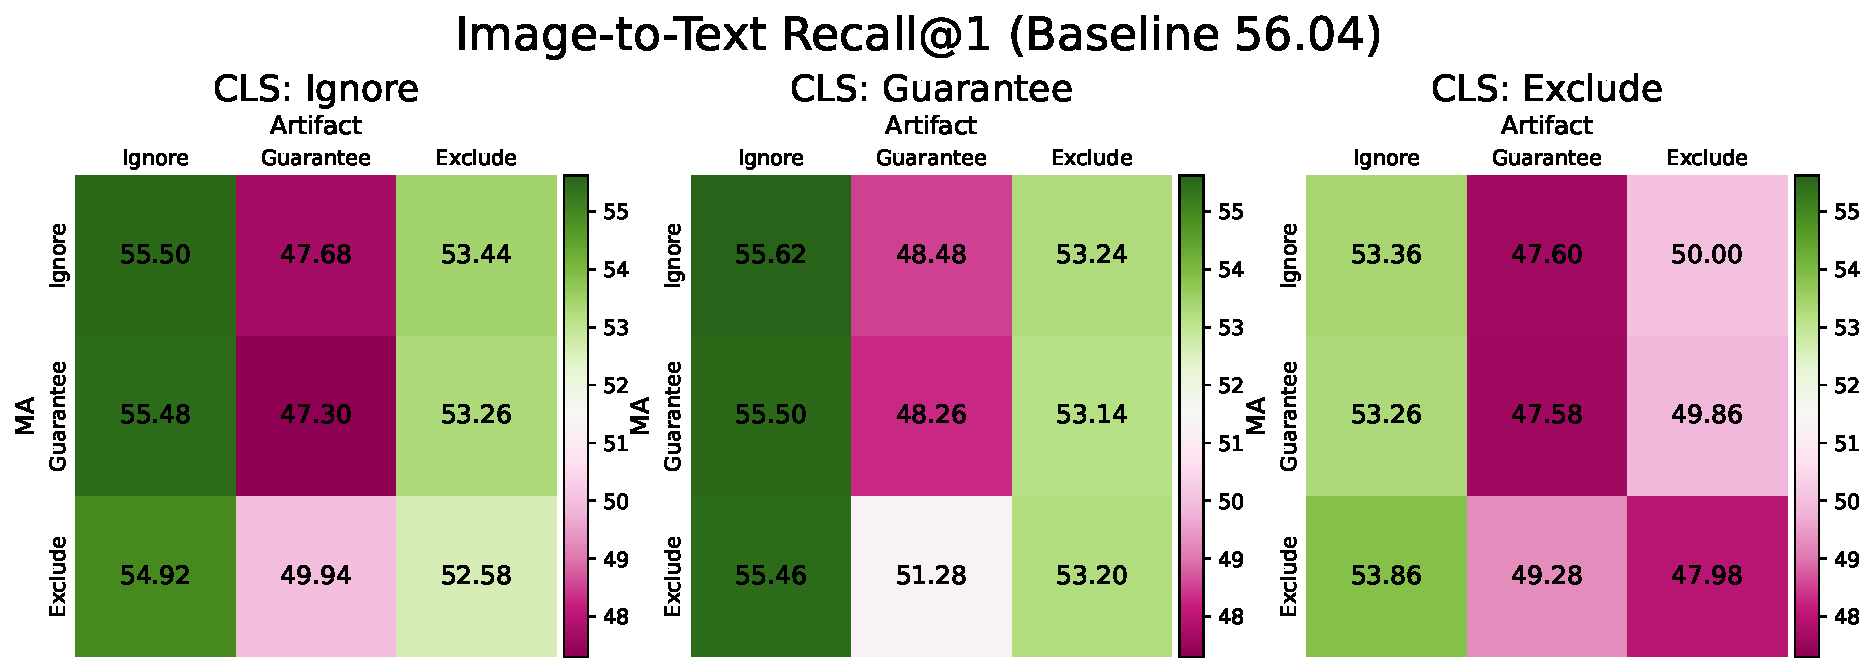
\includegraphics[width=\linewidth]{figs/Image-to-Text_grid.pdf}
        \label{fig:image_to_text_grid_a}
    \end{subfigure}
    \hfill
    \begin{subfigure}[t]{1.0\linewidth}
        \centering
        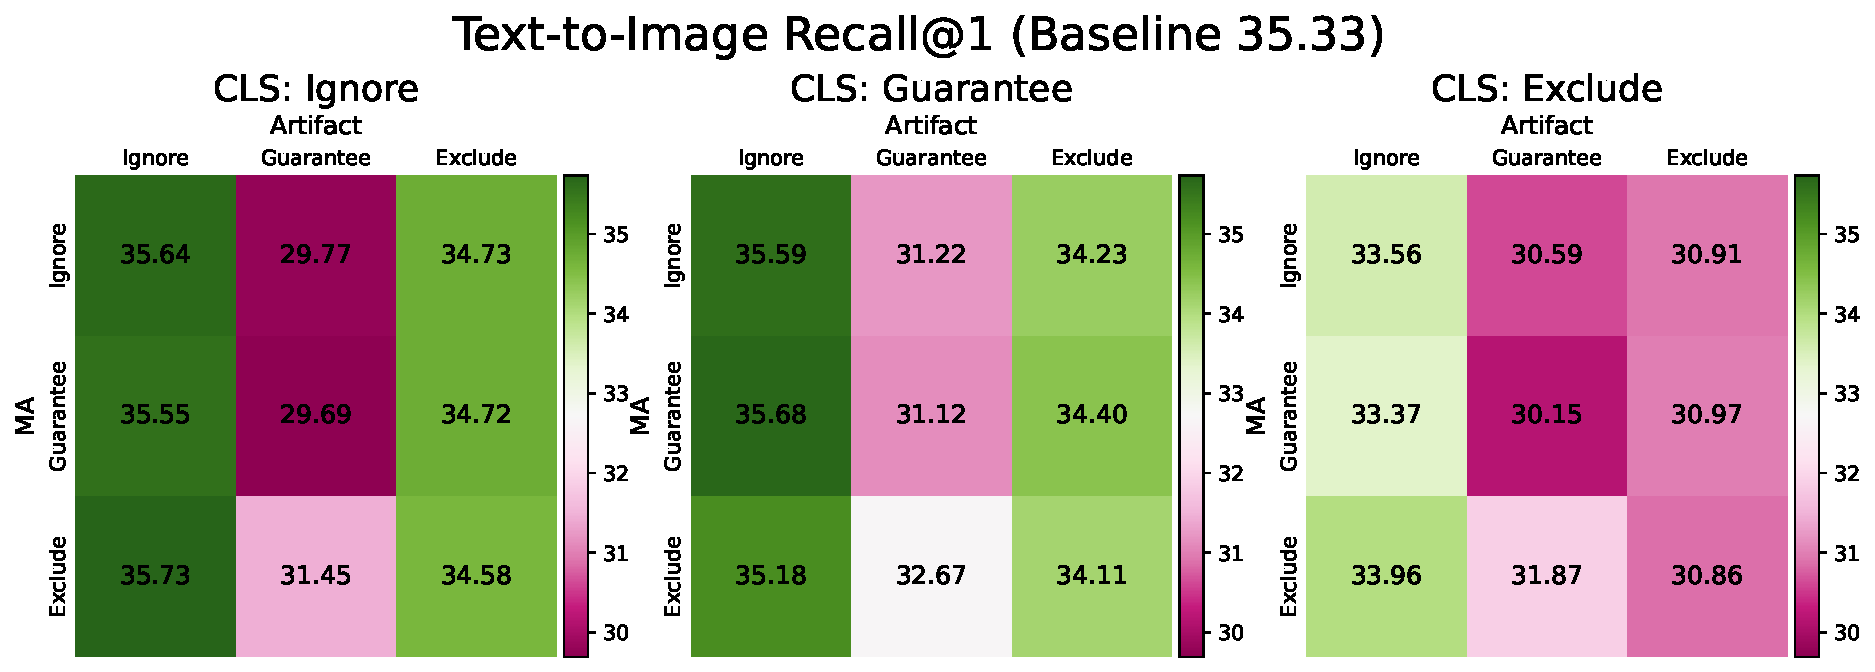
\includegraphics[width=\linewidth]{figs/Text-to-Image_grid.pdf}
        \label{fig:image_to_text_grid_b}
    \end{subfigure}
    \vspace{-1em}
    \caption{COCO retrieval metrics on all $3^3 = 27$ FPS sampling configurations for image-to-text (top) and text-to-image (bottom).}
    \label{fig:coco_recall_subfigs}
\end{figure}


\begin{figure}[b]
    \centering
    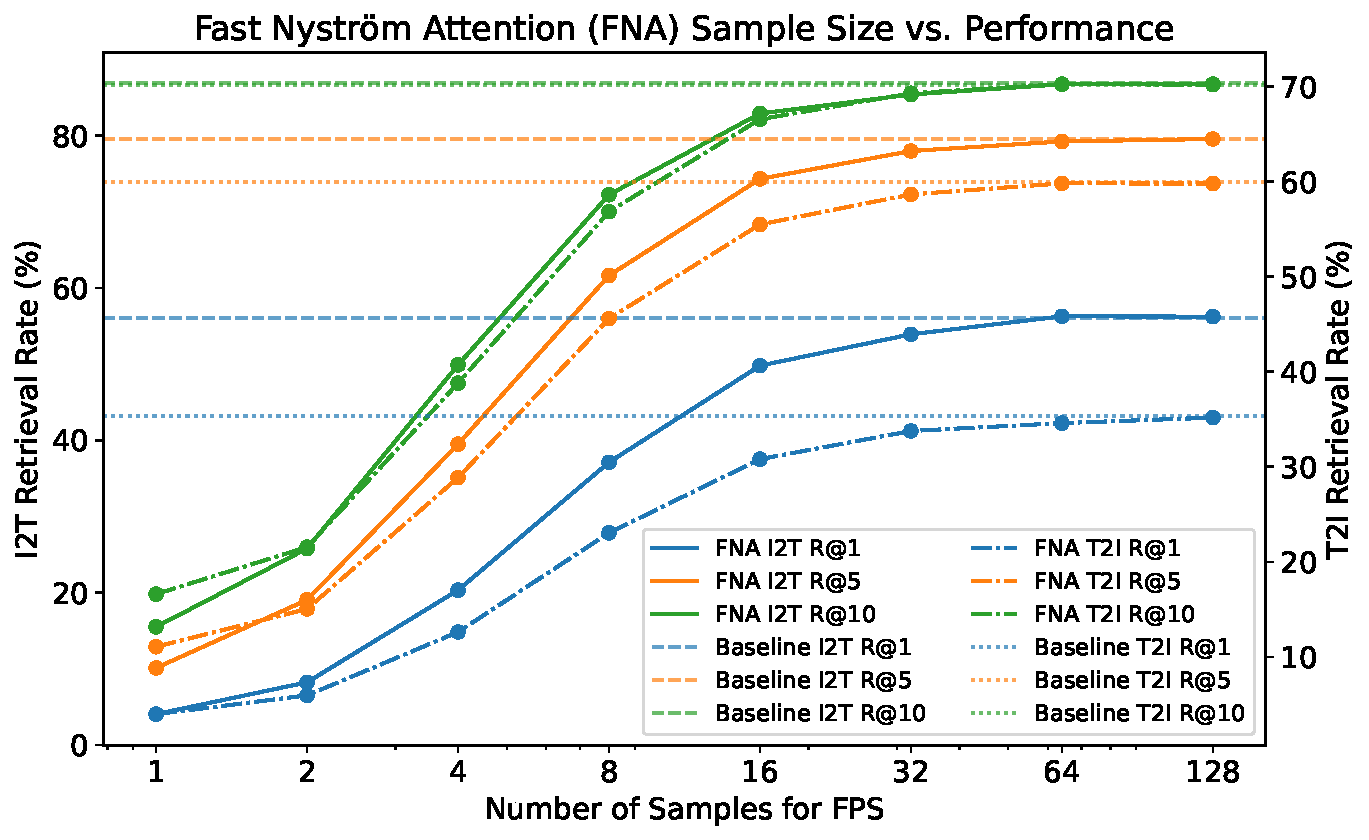
\includegraphics[width=1\linewidth]{figs/fna_sample_size_vs_performance.pdf}
    \vspace{-1em}
    \caption{Furthest point sampling (FPS) sample size vs. performance for COCO retrieval with CLIP ViT L-14 at 224x224px input resolution.}
    \label{fig:fna_sample_size}
\end{figure}



\subsection{Finetuning Comparison with Existing Linear Attention Methods}
\label{sec:appendix_results_linear}

We compare training efficiency of Fast Nystr\"om Attention with existing linear attention methods \cite{choromanski2020performer} \cite{wang2020linformer} \cite{xiong2021nystromformer} by finetuning CLIP ViT L-14 for one epoch on COCO and evaluating retrieval. Validation metrics reported in Table \ref{tab:linear_attn} demonstrate improved performance in both training free and finetuning settings.


\begin{table}[t]
    \centering
    \footnotesize
    \resizebox{0.9\columnwidth}{!}{%
        \begin{tabular}{lccccc}
            \toprule
             & & \multicolumn{2}{c}{Text-to-Image} & \multicolumn{2}{c}{Image-to-Text} \\
            Model & Finetuned & R@1 & R@5 & R@1 & R@5 \\
            \midrule
            Baseline & \xmark & 35.33 & 59.97 & 56.06 & 79.42 \\
            Linformer \cite{wang2020linformer} & \xmark & 0.06 & 0.26 & 0.02 & 0.22 \\
            Performer \cite{choromanski2020performer} & \xmark & 4.28 & 12.07 & 3.76 & 11.06 \\
            FNA+seg. means \cite{xiong2021nystromformer} & \xmark & 32.96 & 57.80 & 49.32 & 74.18 \\ 
            \textbf{FNA+FPS (ours)} & \xmark & 35.91 & 60.43 & 56.52 & 79.32 \\
            \midrule
            Baseline & \cmark & 49.57 & 74.91 & 65.42 & 86.80 \\
            Linformer & \cmark & 18.51 & 42.40 & 22.56 & 47.48 \\
            Performer & \cmark & 41.80 & 69.07 & 53.48 & 79.32 \\
            FNA+seg. means & \cmark & 45.45 & 71.75 & 60.92 & 83.66 \\ 
            \textbf{FNA+FPS (ours)} & \cmark & 48.40 & 73.98 & 64.48 & 86.24 \\ 
            \bottomrule
        \end{tabular}%
    }
    \caption{Validation retrieval performance on COCO using pretrained CLIP ViT L-14 with different linear attention methods applied. We finetune only the QKV projection layers (and down-projection in Linformer). For consistency, we set the down-projection dimension in Linformer and the sample size in Performer and FNA  to 64. We finetune each model with identical hyperparameters on 1 epoch of the COCO training set.}
    \label{tab:linear_attn}
\end{table}



\subsection{Qualitative Results for LLaVa Inference}
\label{sec:appendix_results_llava}

Figure \ref{fig:llava_qualitative} shows qualitative examples of responses generated by LLaVA-NEXT-7B \cite{liu2023llava} on COCO VQA \cite{AgrawalCOCOVQA} prompts, using our Fast Nyström Attention method. These examples illustrate that our approach preserves the semantic quality of the answers while reducing the computational cost.

\begin{figure*}
    \centering
    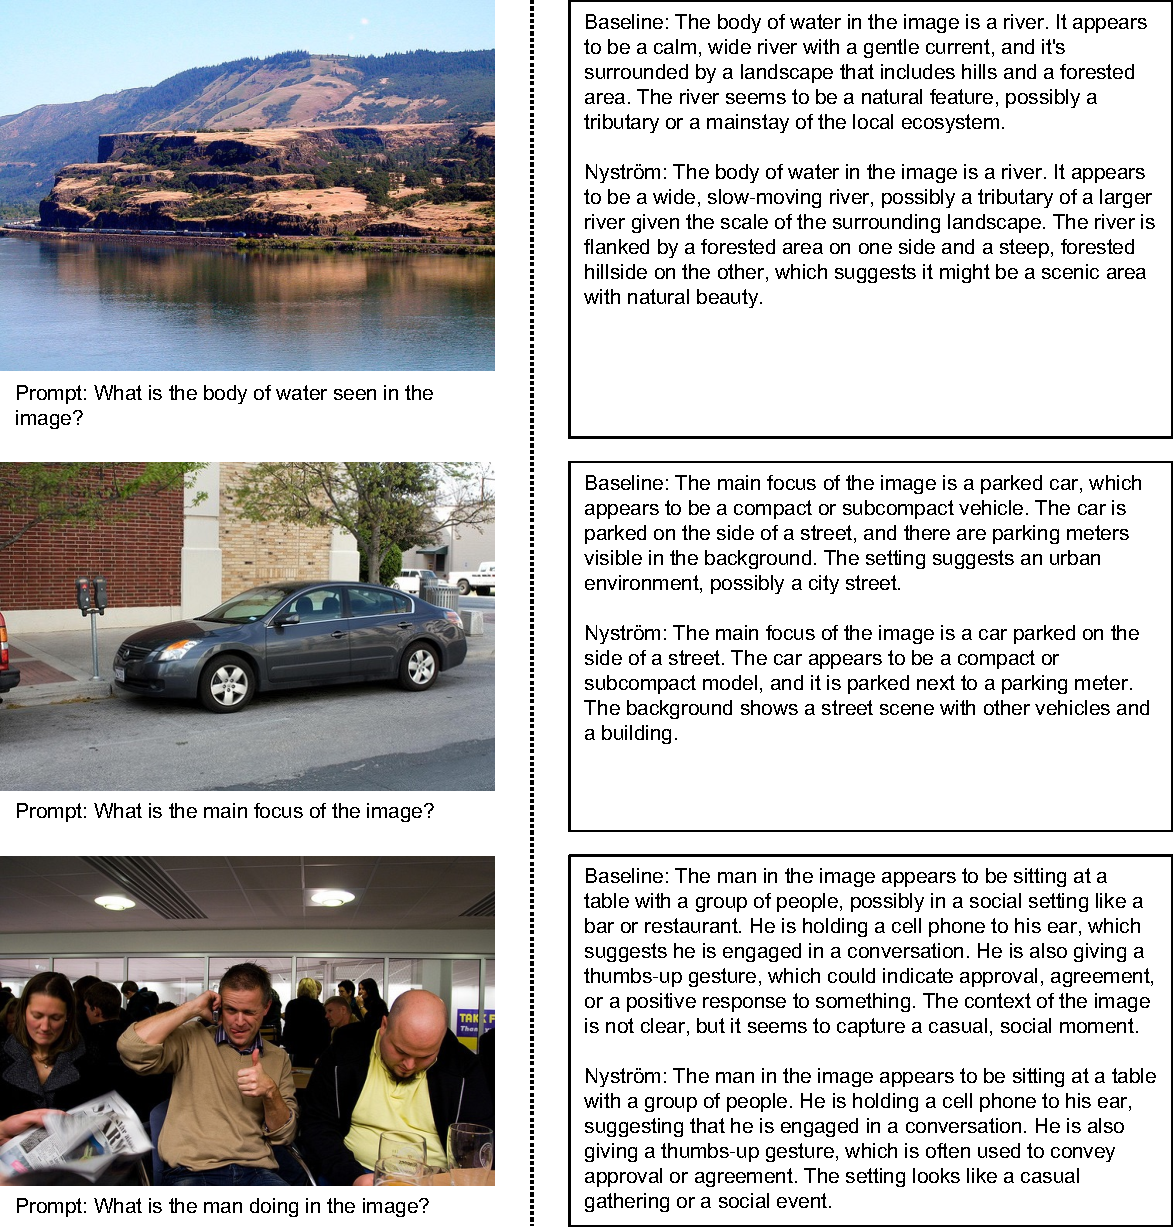
\includegraphics[width=1\linewidth]{figs/llava_qualitative.pdf}
    \caption{Example outputs generated by LLaVA-NeXT-7B \cite{liu2023llava} using input images and text prompts from the COCO VQA \cite{AgrawalCOCOVQA} dataset. We apply Fast Nyström Attention (layers 18 to 32, sample size = 64) to the image tokens in the LLaMA backbone. Greedy decoding is used for generation when comparing against the baseline.}
    \vspace{128in}
    \label{fig:llava_qualitative}
\end{figure*}



\subsection{Sink Token Masking Ablation}
\label{sec:appendix_results_mask_ablation}

In Figure \ref{fig:retrieval_ablation}, we analyze the role sink tokens play at each layer in CLIP ViT-L14 by selectively masking them with the nearest normal token neighbor. When masking sink tokens tokens prior to their formation (\textit{i.e.} masking proto-sink tokens), performance is unaffected as another subset of normal tokens becomes sink tokens. Masking MA tokens after their formation drops performance incrementally since artifact tokens can become massive if needed. Notably, only after removing both MA and artifact tokens at this stage does performance drops considerably, supporting both the importance of sink tokens and the redundant nature of artifact tokens. Removing sink tokens at later layers boosts retrieval metrics as presented in Section \ref{sec:performance_efficiency} and Appendix \ref{sec:appendix_results_mask_gains}.

\begin{figure}
    \centering
    \begin{subfigure}[t]{1.0\linewidth}
        \centering
        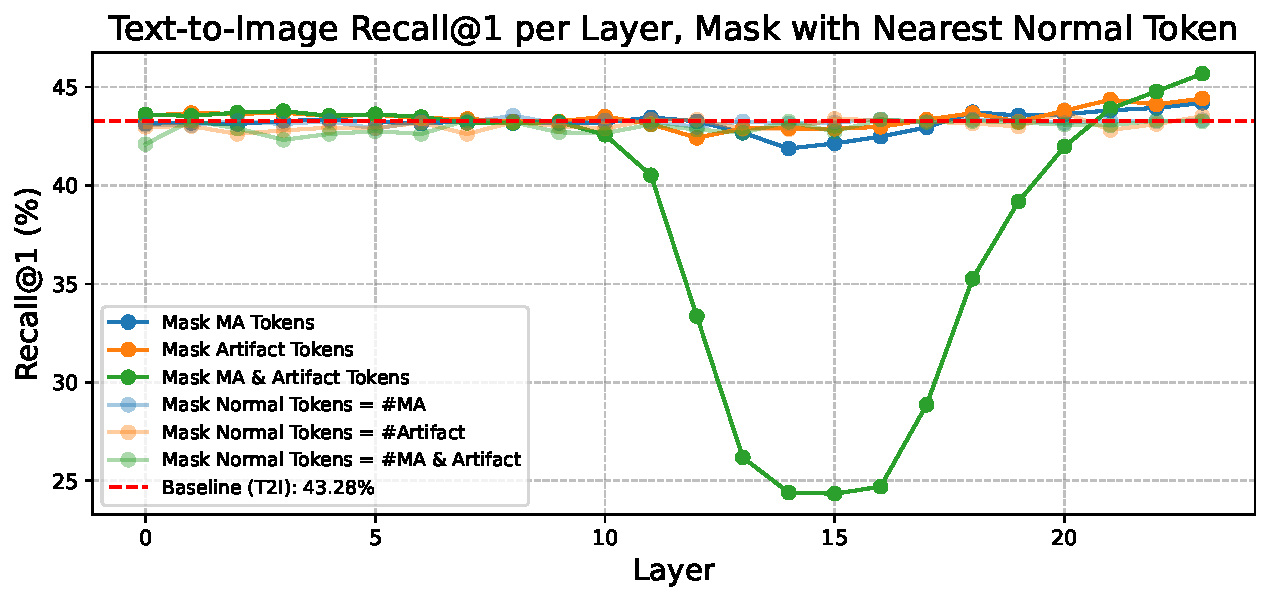
\includegraphics[width=\linewidth]{figs/t2i_replace_with_nearest.pdf}
        \label{fig:t2i_replace}
    \end{subfigure}
    \vspace{0.1cm} % adjust vertical spacing as needed
    \begin{subfigure}[t]{1.0\linewidth}
        \centering
        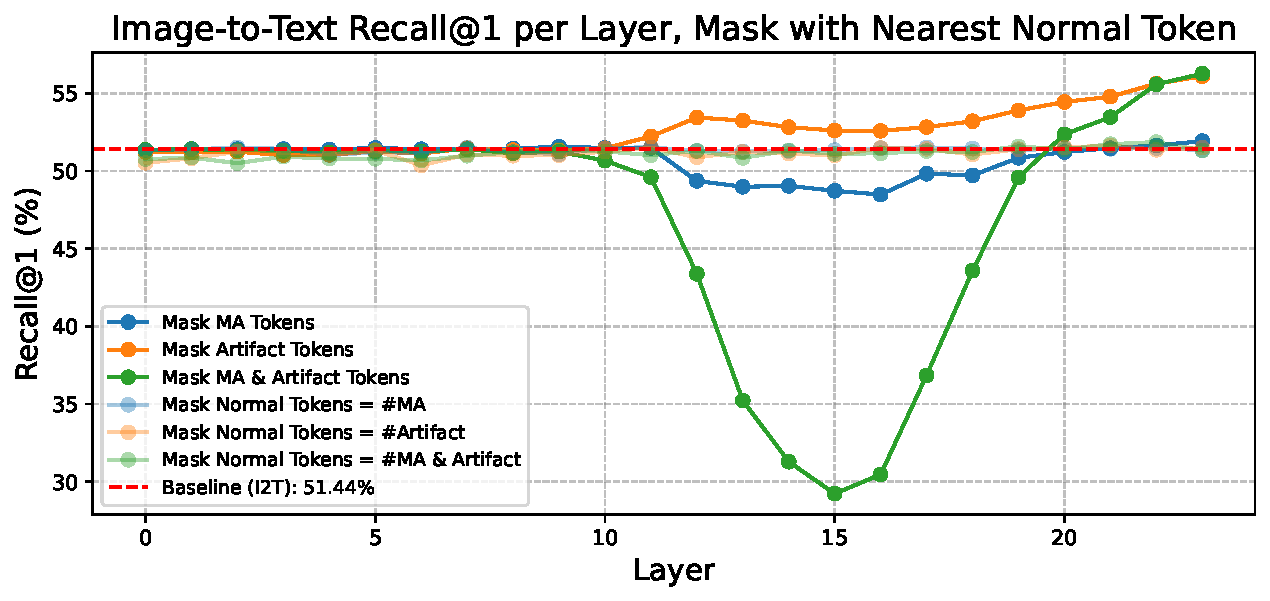
\includegraphics[width=\linewidth]{figs/i2t_replace_with_nearest.pdf}
        \label{fig:i2t_replace}
    \end{subfigure}
    \vspace{-1em}
    \caption{Zero-shot image and text retrieval ablation performed on COCO with pretrained CLIP ViT L-14 show the effect of masking sink tokens at each layer.}
    \label{fig:retrieval_ablation}
\end{figure}


\subsection{Masking Gains on Classification and Segmentation}
\label{sec:appendix_results_mask_gains}

Section \ref{sec:performance_efficiency} demonstrates how masking out massive and artifact tokens in the final layer of pretrained CLIP improves performance on retrieval tasks. Similarly, this masking strategy yields a small boost in zero-shot ImageNet accuracy (Table~\ref{tab:vision_only_results}) with both CLIP and DINOv2. For dense prediction tasks such as semantic segmentation on VOC2012~\cite{pascal-voc-2012} and ADE20k~\cite{zhou2017ade}, masking massive and artifact tokens likewise produces cleaner, more coherent patch features (Figure~\ref{fig:dino_clip_artifacts}) and translates to a minor improvement in segmentation performance.


\begin{table}
\centering
\footnotesize
\resizebox{\columnwidth}{!}{%
\begin{tabular}{lcccccc}
\toprule
 & \multicolumn{2}{c}{ImageNet} & \multicolumn{2}{c}{VOC2012} & \multicolumn{2}{c}{ADE20k} \\
Model & Top1 & Top5 & aACC & mIoU & aACC & mIoU \\
\midrule
CLIP & 75.96 & 94.82 & 90.33 & 66.60 & 69.55 & 34.84 \\
CLIP+masking & \textbf{76.26} & \textbf{94.86} & \textbf{90.59} & \textbf{66.96} & \textbf{69.91} & \textbf{35.09} \\
\midrule
DINOv2 & \textbf{78.62} & 92.91 & 94.12 & 77.54 & 78.65 & 44.48 \\
DINOv2+masking & \textbf{78.62} & \textbf{93.06} & \textbf{94.99} & \textbf{79.65} & \textbf{78.76} & \textbf{44.72} \\
\bottomrule
\end{tabular}%
}
\caption{Vision-only results for pretrained CLIP and DINOv2 ViT L-14. ImageNet \cite{deng2009imagenet} classification evaluation is performed in the zero-shot setting. Segmentation on VOC2012 \cite{pascal-voc-2012} and ADE20k \cite{zhou2017ade} is performed via fitting linear probes to output of the final layers. We show minor but consistent performance gains from masking sink tokens in the final layers.}
\label{tab:vision_only_results}
\end{table}